\documentclass[12pt]{article}
\usepackage[main=russian, english]{babel}
\usepackage[utf8]{inputenc}
\usepackage{amsmath}
\usepackage{booktabs}
\usepackage{float}
\usepackage{geometry}
\usepackage{parskip}
\usepackage{pgf}
\usepackage{siunitx}

\geometry{
    a4paper,
    left=20mm,
    right=20mm,
    top=20mm,
}

\begin{document}

\title{Отчет по лабораторной работе "Изучение спектров атома водорода и молекулы йода"}
\date{}

\maketitle

\section{Цель работы}
Изучить спектр излучения атома водорода (серия Бальмера) и спектр поглощения молекулы йода (серии Деландра).

\section{Теоретические сведения}
\subsection{Спектр излучения водорода}
Для изучения спектр излучения водорода применяется Боровская модель атома
и формула Ридберга:
\begin{equation*}
    \frac{1}{\lambda_{n,m}} = R Z^2 \left( \frac{1}{n^2} - \frac{1}{m^2} \right)
\end{equation*}

При $Z = 1$ (атом водорода) и $n = 2$ (серия Бальмера) получаем:
\begin{equation*}
    \frac{1}{\lambda_m} = R \left( \frac{1}{4} - \frac{1}{m^2} \right) \\
\end{equation*}

Излучение в видимом спектре происходит при
$m = 3, 4, 5, 6$ и обозначается $H_\alpha, H_\beta, H_\gamma, H_\delta$ соответственно.


Измерив $\lambda_m$, можно найти постоянную Ридберга для водорода:
\begin{equation*}
    R = \frac{1}{\lambda_m \left( \frac{1}{4} - \frac{1}{m^2} \right)} \\
\end{equation*}

\subsection{Спектр поглощения йода}
В отличие от отдельных атомов, в молекулах также могут проходить колебательные процессы.
Энергия колебаний также квантуется, поэтому на энергетическом уровне $E_1$
энергия молекулы имеет вид:
\begin{equation*}
    E = E_1 + h \nu_1 (n + \frac{1}{2})
\end{equation*}

На следующем энергетическом уровне $E_2$ энергия молекулы имеет вид:
\begin{equation*}
    E = E_2 + h \nu_2 (m + \frac{1}{2})
\end{equation*}

При поглощении фотона молекула переходит с уровня $E_1$ на уровень $E_2$,
и колебательная энергия также меняется:
\begin{gather*}
    h \nu_{n, m} = (E_2 - E_1) + h \nu_2 (m + \frac{1}{2}) - h \nu_1 (n + \frac{1}{2}) \\
    E_2 - E_1 = h \nu_{\text{эл}}
\end{gather*}

Такой переход с уровня $E_1$ на соседний уровень $E_2$ при фиксированном $n$ называется $n$-той серией Деландра.
Большинство молекул (в силу распределения Больцмана) будут иметь $n = 0, 1$, поэтому лучше всего можно наблюдать
$0$ и $1$ серии Деландра.

\begin{figure}[H]
    \caption{Серии Деландра.}
    \centering
    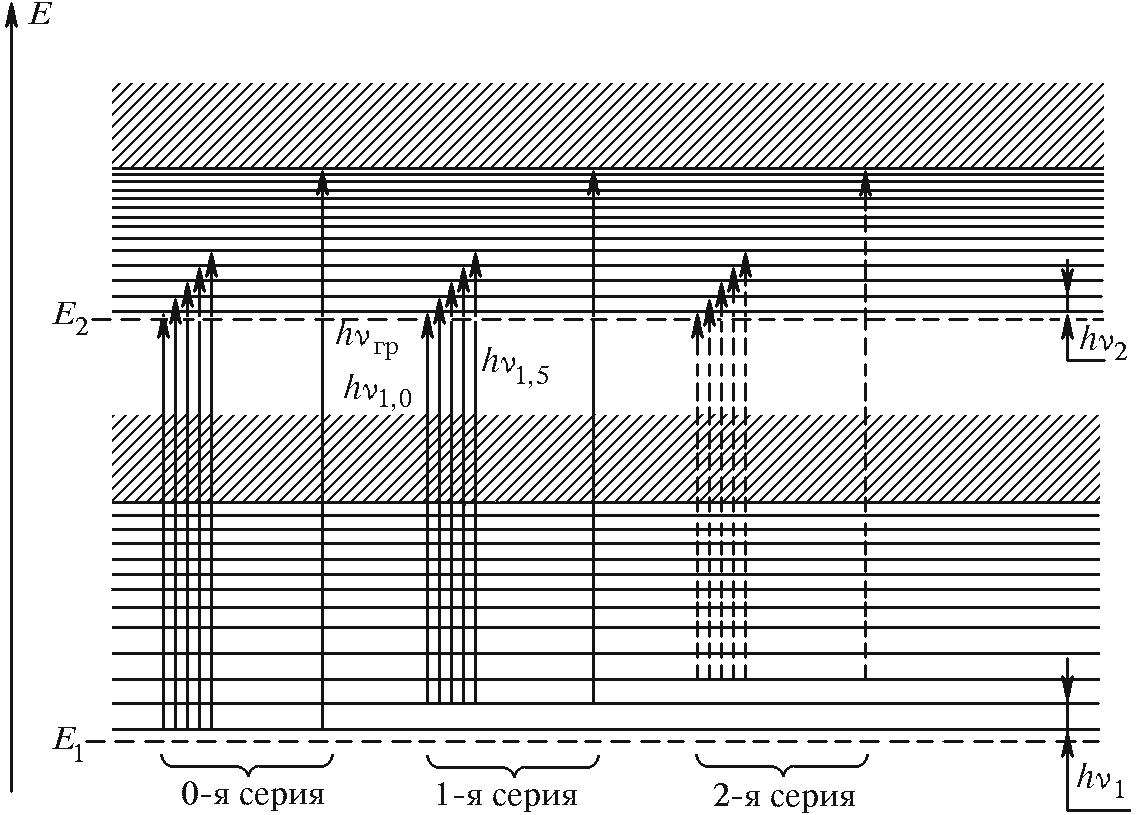
\includegraphics[width=0.75\linewidth]{struct2.png}
\end{figure}

\begin{figure}[H]
    \caption{Вид спектра поглощения.}
    \centering
    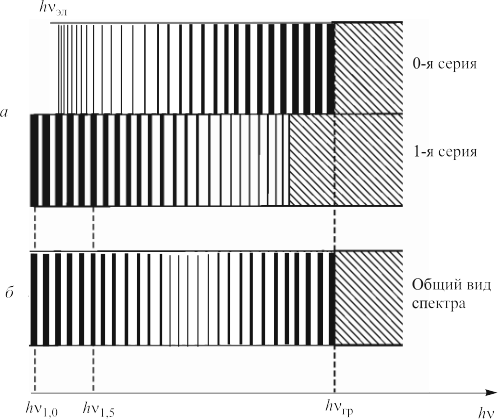
\includegraphics[width=0.6\linewidth]{spec.png}
\end{figure}

При увеличении колебательной энергии растет амплитуда колебаний, и в какой-то момент молекула распадается.
Минимальное количество энергии, которое надо сообщить молекуле при $n = 0$ для ее распада,
называется энергией диссоциации $D_1$.

Частоты выше $\nu_{\text{гр}}$ поглощаются полностью и совпадают с диссоциацией молекулы, находящейся
на уровне $E_2$. Молекула йода на уровне $E_1$ распадается на две атома,
причем энергия одного равна $0$, а другого $E_a$.

\begin{figure}[H]
    \centering
    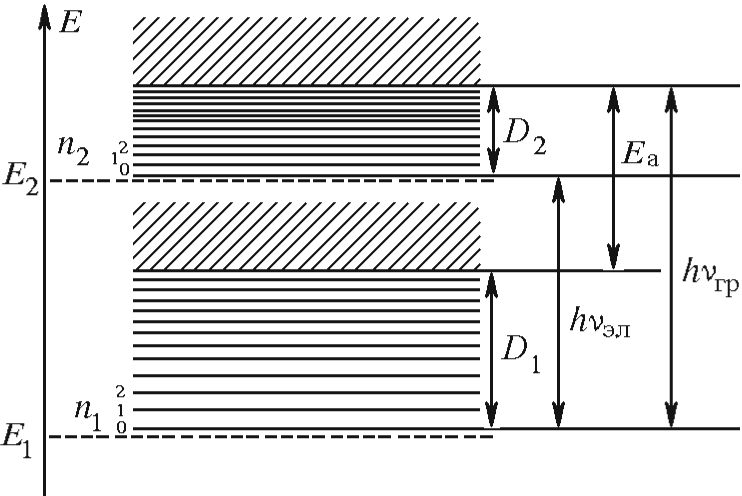
\includegraphics[width=0.5\linewidth]{struct1.png}
\end{figure}

\begin{gather*}
    D_1 + E_a = h \nu_{\text{гр}} \\
    D_1 = h \nu_{\text{гр}} - E_a \\
    D_2 + h \nu_{\text{эл}} = h \nu_{\text{гр}} \\
    D_2 = h \nu_{\text{гр}} - h \nu_{\text{эл}} \\
\end{gather*}

\section{Экспериментальная установка}

Для определения спектров водорода и йода используется проградуированный спектрометр УМ-2. Глядя в окуляр,
барабан $7$ вращается, пока курсор не совпадает с изучаемой линией.
Градуировка спектрометра происходит по неоновой и ртутной лампам, для которых длины волн излучения
известны. Для изучения спектра водорода используется водородная лампа.

\begin{figure}[H]
    \caption{Спектрометр УМ-2.}
    \centering
    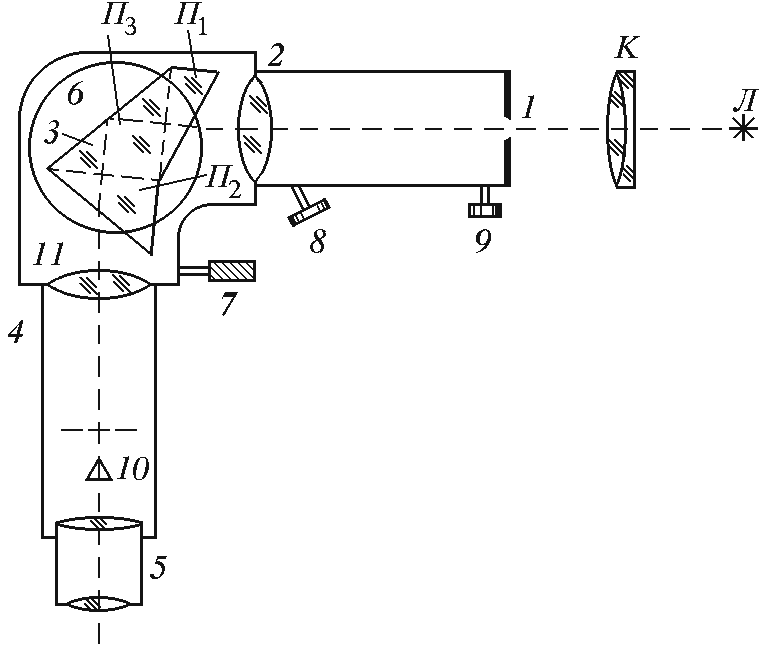
\includegraphics[width=0.5\linewidth]{um2.png}
\end{figure}

\begin{figure}[H]
    \caption{Установка для наблюдения спектра йода.}
    \centering
    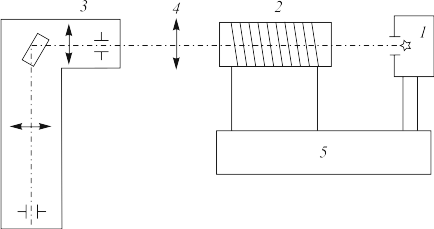
\includegraphics[width=0.5\linewidth]{iodine.png}
\end{figure}

Для наблюдения спектра поглощения йода к установке добавляется кювета с парами йода и лампа накаливания
со сплошным спектром излучения. Для определения кванта энергии колебания $h \nu_2$ на уровне $E_2$ и энергии электронного
перехода $h \nu_{\text{эл}}$ при известном кванте энергии колебания $h \nu_1$ на уровне $E_1$,
можно найти две частоты из 1-ой серии Деландра.
Из структуры спектра видно, что для этого надо найти самую красную видимую линию поглощения (это частота $\nu_{1, 0}$)
и потом от отсчитать от нее $5$ полос (это $\nu_{1, 5}$).
По этим данным теперь можно найти $h \nu_2$ и $h \nu_{\text{эл}}$:
\begin{gather*}
    h \nu_2 = \frac{1}{5} \left( h \nu_{1,5} - h \nu_{1, 0} \right) \\
    E_1 + h \nu_1(1 + \frac{1}{2}) + h \nu_{1, 0} = E_2 + \frac{1}{2} h \nu_2 \\
    h \nu_{\text{эл}} =
        \frac{3}{2} h \nu_1 - \frac{1}{2} h \nu_2 + h \nu_{1, 0} =
        \frac{3}{2} h \nu_1 - \frac{1}{10} h \nu_{1,5} + \frac{11}{10} h \nu_{1, 0}
        \\
\end{gather*}

Если энергия возбуждения $E_a$ известна, для нахождения энергий диссоциации $D_1$ и $D_2$
надо измерить граничную частоту $\nu_{\text{гр}}$, при которой спектр переходит в сплошное поглощение.
Для этого надо найти самую синею видимую линию.

Погрешность показания $n$ барабана $7$ спектрометра УМ-2 $\sigma_n = 2$.

\section{Результаты измерений}
\subsection{Градуировка спектрометра}
\begin{table}[H]
\begin{center}
\caption{Градуировка спектрометра по неоновой лампе.}
\input{neon.tab}
\end{center}
\end{table}

\begin{table}[H]
\begin{center}
\caption{Градуировка спектрометра по ртутной лампе.}
\input{mercury.tab}
\end{center}
\end{table}

Зависимость длины волны излучения от показания барабана я аппроксимировал многочленом 4 степени используя numpy.polyfit()/scipy.optimize.curve\_fit().
Многочлен именно 4 степени наиболее точно описывает полученные данные.
Я также пробовал вместо многочлена использовать гиперболу, но для нее не получилось подобрать коэффициенты.

\begin{figure}[h!]
    \centering
    \input{grad.pgf}
\end{figure}

\begin{gather*}
    \lambda(n) = P_4(n) = a_4 n^4 + a_3 n^3 + a_2 n^2 + a_1 n + a_0 \\
    \sigma_\lambda = \sqrt{\left( \frac{\partial P_4}{\partial n} \sigma_n \right)^2 + J \Sigma J^T } \\
    J = \frac{\partial P_4}{\partial a}, \Sigma - \text{ковариационная матрица для коэффициентов $P_4$}
\end{gather*}

\subsection{Спектр водорода}
\begin{gather*}
    \frac{1}{\lambda_m} = R \left( \frac{1}{4} - \frac{1}{m^2} \right) \\
    R = \frac{1}{\lambda_m \left( \frac{1}{4} - \frac{1}{m^2} \right)} \\
\end{gather*}

\begin{table}[H]
\begin{center}
\caption{Серия Бальмера.}
\input{balmer.tab}
\end{center}
\end{table}

Здесь $\lambda_{ref}$ - табличное значение длины волны излучения.

Проведем усреднение $R$:
\input{R}
Табличное значение $R_{ref} = 1.0967$. Полученное экспериментальным путем $\overline{R}$ совпадает с ним.
Каждая линия по отдельности также соответствует этому значению, кроме $H_\alpha$.
Возможно это связанно с неточным снятием показания спектрометра.

\subsection{Спектр йода}
\begin{gather*}
    h \nu_2 = \frac{1}{5} \left( h \nu_{1, 5} - h \nu_{1, 0} \right) \\
    h \nu_{1, m} = h \nu_{\text{эл}} + h \nu_2 (m + \frac{1}{2}) - \frac{3}{2} h \nu_1 \\
    h \nu_{\text{эл}} =
        \frac{3}{2} h \nu_1 - \frac{1}{2} h \nu_2 + h \nu_{1, 0} =
        \frac{3}{2} h \nu_1 - \frac{1}{10} h \nu_{1, 5} + \frac{11}{10} h \nu_{1, 0} \\
    D_1 = h \nu_{\text{гр}} - E_a \\
    D_2 = h \nu_{\text{гр}} - h \nu_{\text{эл}} \\
\end{gather*}

Проанализируем погрешность этого опыта. При определении последней линии на глаз, можно ошибиться на $\sigma_k = 1$ линию.
Для $h \nu_{\text{гр}}$ это означает (если пренебречь ангармонизмом), что к $\sigma_{h \nu_{\text{гр}}}$ надо добавить $\sigma_k h \nu_2$.
Аналогично для $h \nu_{\text{эл}}$, что видно из формулы.

\begin{table}[H]
\begin{center}
\caption{Спектр поглощения йода.}
\input{iodine.tab}
\end{center}
\end{table}

\begin{table}[H]
\begin{center}
\caption{Энергии йода.}
\input{energies.tab}
\end{center}
\end{table}

Полученные экспериментальным путем значения $h \nu_{\text{гр}}$ и $D_1$ соответствуют табличным,
но $D_2$ своему табличному значению не соответствует, что указывает на возможный большой ($\approx 10$ полос) промах в определении $\nu_{1, 0}$.

\section{Заключение}
Изучены спектр излучения водорода и спектр поглощения йода. Удалось точно померить постоянную Ридберга для водорода.
Получилось определить энергию части переходов в молекуле йода при поглощении излучения.

\end{document}
